\begin{tikzpicture}[>=latex, x=1.15cm, y=0.8cm]
  \draw[->] (0,0) -- (8.2,0) node[right] {$t$};
  \draw[->] (0,0) -- (0,5) node[above] {$f$};
  \draw[dotted] (0,4) -- (8,4); 
  \node[left] at (0,4) {$f_{\max}$}; \node[left] at (0,0) {$f_{\min}$};
  % gesendet
  \draw[very thick, blue!70!black] (0,0) -- (3,4) -- (6,0) -- (7.5,2) node[right, font=\small] {gesendet};
  % Echo
  \draw[very thick, red, dashed] (0.5,0.3) -- (3.5,4.3) -- (6.5,0.3) -- (7.5,1.63) node[right, font=\small, yshift=-8pt] {Echo};
  % Delta t, Delta f am Anfang
  \draw[<->] (0,-0.5) -- (0.5,-0.5) node[midway, below, font=\small] {$\Delta t=\tfrac{2s}{c}$};
  \draw[dotted] (0.5,-0.5) -- (0.5,0.3);
  % f^- auf der Steigung
  \draw[<->, thick] (1.5,1.633) -- (1.5,2) ;
  \node[right, font=\small] at (1.5,1.55) {$f^{-}=k\Delta t-\Delta f$};
  % f^+ auf dem Abstieg
  \draw[<->, thick] (4.5,2) -- (4.5,2.967);
  \node[right, font=\small, fill=white, inner sep=1pt] at (4.7,2.4) {$f^{+}=k\Delta t+\Delta f$};
  % Steigung k
  \node[font=\small, blue!70!black] at (0.9,3.0) {Steigung $k$};
\end{tikzpicture}
